%\documentclass{winnower}
\documentclass{article}
\usepackage{amssymb}
\usepackage{graphicx}
\usepackage[margin=0.9in]{geometry}
\begin{document}

\title{A Comparative Study of Generative Adversarial Networks Towards Automatic Image Colorization}

\author{Cameron Fabbri}
\date{4/24/2017}

\maketitle

%\begin{abstract}
%We provide an overview of Generative Adversarial Networks as a class of generative models for
%image generation, and discuss how they can be applied towards the task of automatic image colorization. 
%We first give a brief overview of Deep Learning and the recent advances in generative models.
%We then discuss several varients of Generative Adversarial Networks, the problems they pose during training,
%and theoretical methods towards stabalizing training.
%\end{abstract}


%-------------------------------------------------%
\section{Introduction}
%-------------------------------------------------%
Deep learning has recently shown impressive results towards various problems in multiple domains such as speech recognition,
image classification, image segmentation, and reinforcement learning []. Until recently, much of the focus was towards
discriminative models, which aim to map a high-dimensional input, such as an image, to a class label. Deep generative models,
such as Deep Botlzmann Machines, Deep Belief Networks, and Autoencoders have not had the same level of success.
Generative Adversarial Networks (GANs)[1] are a class of generative models that have shown great success in generatig realistic
images. Despite their success, they are known to be very difficult to train, and are extremely sensitive to modifications.
For this reason it is not yet straightforward to directly apply them towards different problems or problems of a different domain.\newline

\noindent Since their introduction in 2014, there have been several large contributions made towards stabalizing and understanding
the training process of GANs. I will be focusing on implementing and comparing four different methods used for training GANs towards
the original problem of image generation. With these implemented, I apply their methods towards our goal to automatically
colorize grayscale images. The four different variants of GANs I will be focusing on are the original GAN formulation [1], Least Squares
GANs (LSGANs) [6], Energy-Based GANs (EBGANs) [4], and Wasserstein GAN (WGAN) [5]. The papers I will be discussing are [1,2,3,4,5,6], with additional
references to others not listed here. The original GANs paper [1] provides a novel method towards generating images with the use of an
adversarial loss, where both the generator and discriminator networks are multilayer perceptrons. Deep Convolutional GANs (DCGANs) [2]
bridge the gap between recent advances in deep learning and GANs by introducing deep convolutional generative adversarial networks. The architechture they contribute
is used in "pix2pix" [3], which approaches the problem of translating images from one domain to the other, in [4] which views the discriminator
as an energy function, in [5] which proposes to minimize an approximation of the Earth Mover distance, and in [6], which adopt the
least squares loss function in attepmt to overcome the vanishing gradient problem commonly seen with GANs.

%-------------------------------------------------%
\section{Background and Related Work}
%-------------------------------------------------%

%-------------------------------------------------%
\subsection{Deep Learning}
%-------------------------------------------------%
Deep learning is a class of machine learning algorithms that use one or more \textit{hidden layers} between the input and output
to learn a heirarchy of concepts, often referred to as \textit{deep neural networks} (DNN).
In a feedforward network, or multilayer perceptron (MLP), each successive layer uses the output
from the previous layer as input, and uses an activation function, such as a logistic function, to obtain a new representation of the input. To
learn the set of weights and biases connecting successive layers, the error is propagated backwards through the network in order to optimize a
given objective function. This process is known as \textit{backpropogation}. Backpropogation is used in conjunction with an optimization method,
such as gradient descent, to effeciently compute the gradients by propogation from the output to input. This allows multi-layer networks to learn
a non-linear mapping from copious amounts of data. Because of the large amount of data needed to effectively train DNNs, \textit{stochastic gradient descent}
is often used via batches of data, which amounts to computing the gradient on a mini-batch of training samples. Recent advances in GPUs have
provided massive speedups in training due to their ability to parallelize the many operations in a DNN. \newline

%-------------------------------------------------%
\subsection{Convolutional Neural Networks}
%-------------------------------------------------%
\noindent The most common type of DNN for visual data is the Convolutional Neural Network (CNN), which is designed specifically for
multidimensional data such as images. CNNs incorporate three powerful techniques in order to achieve some degree of scale and shift invariance.
The first is the use of shared weights, which stems from the idea that a feature detector used in one part of an image is almost certainly useful in
other parts of the image. This also allows networks to reduce the number of parameters to avoid the curse of dimensionality. The second is the use of
local receptive fields. A kernel or filter is \textit{convolved} across the entire
image to produce a \textit{feature map}. Each pixel in the resulting feature map is the result of the kernel convolved with a small area in the input.
The use of local receptive fields allow earlier layers in the network to learn low-level features such as edges or corners, which can then be combined
in successive layers throughout the network to learn high-level features. The third technique is various forms of subsampling, such as the use of pooling
layers, which provide a form of nonlinear downsampling. Subsampling is performed to reduce the dimensionality of the internal representation. \newline

\noindent While the size of the output in a MLP is independent of the size of its input,
the height and width of the resulting feature maps are dependent on the size and stride of the kernel. The number of feature maps or \textit{depth} of the
resulting layer (which corresponds to the \textit{width} of the network as a whole) however, is arbitrary. Clearly, there are many different opitions to be chosen,
such as the size of the kernel, the stride of the kernel, depth of the . When designing a CNN, many rely on heuristics, as well as theorectical
design principles as shown in [inception paper]. An example CNN architecture is shown in Figure 1. \newline

%-------------------------------------------------%
\subsection{Deep Generative Models}
%-------------------------------------------------%
\noindent Much focus has been put on CNNs as a discriminative model, learning a function to map some input data to some desired output label. In other words,
they learn the conditional distribution $P(y|x)$. The rest of this paper is focused on \textit{generative} models, which instead learn the joint
probability of the input data and labels. They attempt to model the data directly by learning $P(x,y)$. Autoencoders, Deep Boltzmann Machines, and
Deep Belief Nets are some examples of these class of models. Generative models are usually based on some generator network $G$, that takes as input
a random variable $z$ sampled from some distribution, e.g $z \sim \mathcal{N}(0,1)$, and outputs a sample $x$. \newline

\noindent Generative models, as the name suggest, attempt to generate new data similar to existing data. Generative models have been shown to perform
well on many tasks such as inpainting, image denoising, and video generation. Autoencoders have been a popular form of generative model because of their
ability to approximate some distribution of observed data, such as imagery. A simple autoencoder setup may be to learn an encoding $z$ over a set of images,
$\mathcal{X}$, with $z$ being of a much lower dimension than that of $X \in{\mathcal{X}}$. A training procedure for a setup such as this is as follows.
An image $X \in{\mathbb{R}^{m\times n}}$ is encoded through an encoder CNN to some latent variable $z \in{\mathbb{R}^{d}}$, which is then used as input to a
decoder CNN to produce $X' \in{\mathbb{R}^{m\times n}}$. A loss function, such as $L_2$ is then used to compare the two, and the error is propogated back through
the networks. To produce a new sample, a random variable $z' \sim \mathcal{N}$ can be used as input to the generator network in place of an encoded $z$. 
An open research problem is to determine an appropriate loss function. $L_2$ and $L_1$ often result in blurry images, and may not be a correct metric for
visual quality. A recent class of generative models proposes to instead use an \textit{adversarial} loss in place of existing loss functions in the form of
a network.


\begin{figure}[!htb]
   \begin{center}$
      \begin{array}{cccc}
         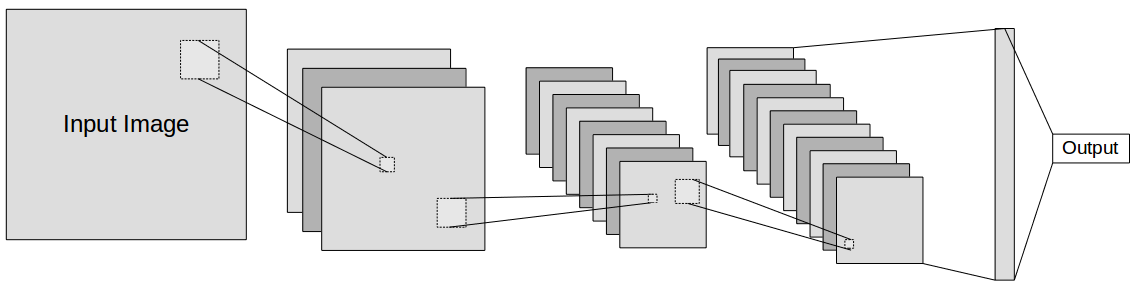
\includegraphics[width=3in]{cnn}
      \end{array}$
   \end{center}
   \caption{An example of a Convolutional Neural Network}
\end{figure}

\pagebreak

%-------------------------------------------------%
\section{Generative Adversarial Networks}
%-------------------------------------------------%
\noindent Generative Adversarial Networks (GANs) [1] are a recent class of generative models that are based on a game theory scenario in which a generator
network is competing against an adversary. The goal is to train a generator network to generate samples that are indistinguishable from the true data $p_{data}$
by mapping a random input variable $z \sim p_z$. This mapping can be represented as $G(z;\theta_g)$, where $G$ is a MLP with weights $\theta_g$, and $z$ is a random
variable sampled from some distribution, e.g $z \sim \mathcal{N}(0,1)$. The discriminator, $D(\textbf{\textit{x}}; \theta_d)$ is represented by a second MLP with weights
$\theta_d$, and outputs a scalar representing the probability that a sample $\textbf{\textit{x}}$ came from $p_{data}$ rather than from $G$. The two networks are trained
simultaneously, with $D$ being trained to correctly predict whether or not a sample came from $p_{data}$ or from $G$, and $G$ being trained to fool $D$ by minimizing $log(1-D(G(z)))$.
This can be represented by the following value function:

\[\min\limits_{G}\max\limits_{D} V(D,G) = \mathbb{E}_{x \sim p_{data(x)}} [logD(\textbf{\textit{x}})] + \mathbb{E}_{z \sim p_z(z)}[log(1 - D(G(z)))]\]

\noindent As discussed in [3], GANs have been shown to optimize the Jensen-Shannon divergence (JSD), which is a symmetrized and smoothed version of the Kullback-Leibler
(KL) divergence. 

GANs have the attractive property that in theory, blurry images should be rejected by the discriminator for looking unrealistic. However, they are extremely
difficult to train, often resulting in mode collapse, where either the generator or discriminator largely outperforms the other. 


%-------------------------------------------------%
\subsection{Conditional Generative Adversarial Networks}
%-------------------------------------------------%
Conditional GANs (cGANs) introduce a simple method to condition image generation on some extra information $y$ (e.g a class label). This is done by simply feeding
$y$ to the generator and discriminator networks.



%-------------------------------------------------%
\subsection{Deep Convolutional GANs}
%-------------------------------------------------%


%-------------------------------------------------%
\subsection{Least Squares GANs}
%-------------------------------------------------%


%-------------------------------------------------%
\subsection{Energy-Based GANs}
%-------------------------------------------------%	 


%-------------------------------------------------%
\subsection{Wasserstein GANs}
%-------------------------------------------------%


%-------------------------------------------------%
\section{Colorization}
%-------------------------------------------------%
We now show how adversarial networks can be used for generating a plausible color version of a grayscale image.
The problem is set up as a cGAN, where the generator and descriminator are both conditioned on the grayscale image.






\bibliographystyle{abbrvnat}
\noindent [1] Goodfellow, Ian, Yoshua Bengio, and Aaron Courville. Deep learning. MIT Press, 2016. \newline
\noindent [2] Radford, Alec, Luke Metz, and Soumith Chintala. "Unsupervised Representation Learning with Deep Convolutional Generative Adversarial Networks." ICLR (2016): https://arxiv.org/abs/1511.06434.
\noindent [3] Isola, Phillip, Zhoe, Efros. "Image-to-image translation with conditional adversarial networks." arXiv preprint arXiv:1611.07004 (2016).
\noindent [4] Zhao, Junbo, Michael Mathieu, and Yann LeCun. "Energy-based generative adversarial network." arXiv preprint arXiv:1609.03126 (2016).
\noindent [5] Arjovsky, Martin, Soumith Chintala, and Léon Bottou. "Wasserstein gan." arXiv preprint arXiv:1701.07875 (2017).
\noindent [6] Mao, Xudong, et al. "Least squares generative adversarial networks." arXiv preprint ArXiv:1611.04076 (2016).


\noindent [7] Graves, Alex, and Navdeep Jaitly. "Towards End-To-End Speech Recognition with Recurrent Neural Networks." ICML. Vol. 14. 2014.
\noindent [8] Arjovsky, Martin, and Léon Bottou. "Towards principled methods for training generative adversarial networks." NIPS 2016 Workshop on Adversarial Training. In review for ICLR. Vol. 2016. 2017.
\bibliography{winnower_template}

\appendix

\section{Appendix}
Here we show 


\end{document}
